\section{DriveWorld}	
Consider a sequence of observed $T$ video frames denoted as $o_{1:T}$, captured by multi-view cameras, along with their corresponding expert actions, $a_{1:T}$ and 3D occupancy labels $y_{1:T}$ which can be acquired with the aid of LiDAR point clouds and pose data, we aim to learn a compact spatio-temporal BEV representation via world model that predicts current and future 3D occupancy given the past multi-camera images and actions. As shown in Fig.~\ref{fig:flowchart}, the designed world model consists of an Image Encoder, a 2D to 3D View Transform (\eg, Transformers~\cite{detr3d}, LSS~\cite{lss} techniques), a Memory State-Space Model which consists of a Dynamic Memory Bank module to learn the temporal-aware latent dynamics and a Static Scene Propagation module to learn the spatial-aware latent statics, a Decoder to predict the actions and 3D occupancy, and a Task Prompt to condition the feature extraction for different tasks. 

\subsection{Memory State-Space Model}

As autonomous vehicle moves, it sequentially conveys two types of information within its observations: the temporal-aware information linked to alterations in the scene due to object mobility, and the spatial-aware information associated with scene context~\cite{contextwm}. As illustrated in Fig.~\ref{fig:mssm}, to address these dynamic agents and spatial scenes separately for 4D pre-training, we propose the Dynamic Memory Bank module for temporal-aware latent dynamics and the Static Scene Propagation module for spatial-aware latent statics. Next, we will begin by introducing the probabilistic model for temporal modelling, followed by detailed presentations of the Dynamic Memory Bank module and Static Scene Propagation module.

\paragraph{Probabilistic Modelling.}
To imbue the model with the capability for temporal modelling, we first introduce two latent variables $(h_{1:T}, s_{1:T})$, where $h_t$ represents the history and $s_t$ signifies the stochastic state. $h_t$ is updated with the past histories $h_{1:t-1}$ and stochastic states $s_{1:t-1}$. 

When images are observed, current scene perception can be obtained by utilizing past and current images. However, when predicting the future, in the absence of input images, we rely solely on past histories and states $(h_{1:t-1}, s_{1:t-1})$ to predict the future states. This predictive process is akin to the probabilistic generative models~\cite{vae}. For predicting future, we follow Recurrent State-Space Model~\cite{plas_wm} and construct both the posterior state distribution $q(s_t|o_{\leq t},a_{< t})$ and the prior state distribution $p(s_t|h_{t-1},s_{t-1})$. The objective is to match the prior distribution (the anticipated outcome based on past histories and states) with the posterior distribution (the outcome derived from observed multi-camera images and actions)~\cite{mile}.  

Considering the high dimensionality of BEV features, we transform them into a 1D vector $x_t\in \mathbb{R}^{512}$ and subsequently sample the Gaussian distribution from $(h_t, a_{t-1},x_t)$ to generate the posterior state distribution:

%%\vspace{-1em}
\begin{footnotesize} 
	\begin{equation} \label{post}
	q(s_t|o_{\leq t},a_{< t})\backsim \mathcal{N}(\mu _{\phi }(h_t,a_{t-1},x_t),\sigma _{\phi }(h_t, a_{t-1},x_t)\textbf{\textit{I}}),
	\end{equation} 
\end{footnotesize}
where $s_t$ is parameterised as a normal distribution with diagonal covariance and the initial distribution is set as $s_1\backsim \mathcal{N}(0,\textbf{\textit{I}})$. $(\mu _{\phi }, \sigma _{\phi })$ are multi-layer perceptrons that parametrise the posterior state distribution. 

In the absence of observed images, the model derives the prior state distribution based on historical information and predicted action:

%%\vspace{-1em}
\begin{footnotesize} 
	\begin{equation} \label{prior}
	p(s_t|h_{t-1},s_{t-1})\backsim \mathcal{N}(\mu _\theta (h_t,\hat{a}_{t-1}),\sigma_\theta (h_t,\hat{a}_{t-1})\textbf{\textit{I}}),
	\end{equation} 
\end{footnotesize}
where $(\mu _{\theta }, \sigma _{\theta })$ parameterizes the prior state distribution. $\pi _\theta$ is the policy network for predicting action $\hat{a}_{t-1}$ with past history $h_{t-1}$ and state $s_{t-1}$. Following MILE~\cite{mile}, we utilize MLP for action prediction, including velocity and steering.
%%\vspace{-1em}
\paragraph{Dynamic Memory Bank.}
\begin{figure}[t]
	\centering
	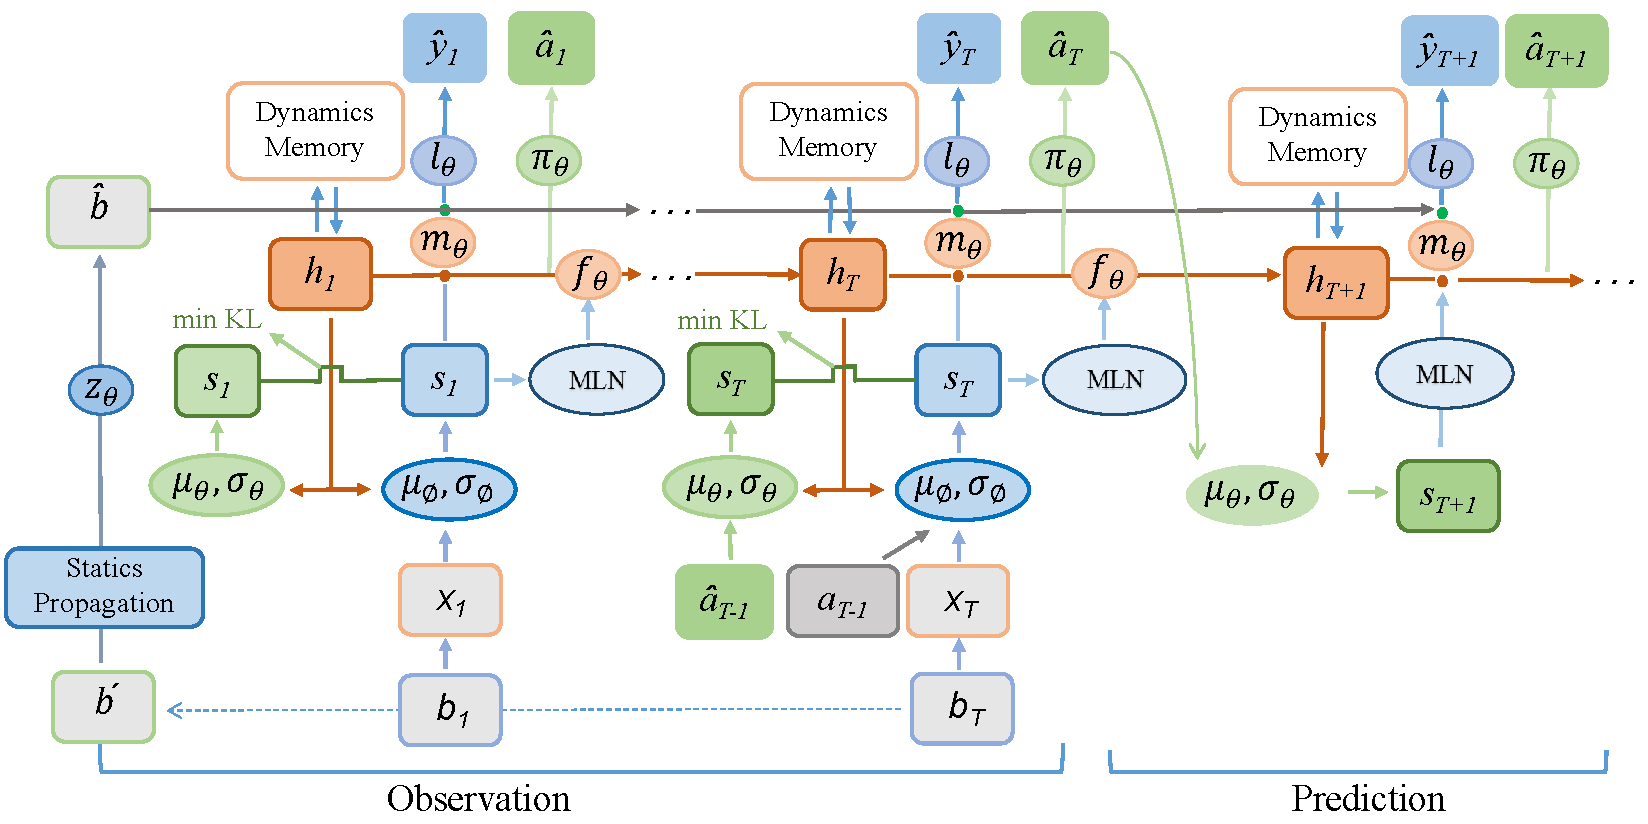
\includegraphics[width=0.48\textwidth]{figures/mssm}
	\caption{Overall architecture of proposed the Memory State-Sapce Model (MSSM). MSSM divides the transmitted information into two categories: temporal-aware information and spatial-aware information. The Dynamic Memory Bank module utilizes motion-aware layer normalization (MLN) to encode temporal-aware attributes and engages in information interaction with the dynamically updated memory bank. Meanwhile, the Static Scene Propagation module employs BEV features to represent spatial-aware latent statics, which are directly conveyed to the decoder.
	}
	%%\vspace{-1em}
	\label{fig:mssm}
\end{figure}
In the process of temporal information propagation, we aim to account for the movement of objects by incorporating motion parameters.   Following StreamPETR~\cite{streampetr}, we introduce motion-aware layer normalization (MLN) into the latent dynamics propagation process. We define $K$ moving objects and estimate their velocities. The motion attributes consist of velocity $v$, and relative time interval $\Delta t$. $(v, \Delta t)$ are flattened and converted into affine vectors $\gamma $ and $\beta$ through two linear layers $(\xi_1, \xi_2)$: $\gamma = \xi_1(v, \Delta t),
\beta = \xi_2(v, \Delta t).$ 
Then an affine transformation is executed to yield the motion-aware latent stochastic state, denoted as $\tilde{  s}_{t} = \gamma \cdot LN(  s_{t}) + \beta.$
With the motion of the vehicle, the deterministic history $  h_t$ can establish a dynamic memory bank $  h_{1:t}$. The refined deterministic history $\tilde{  h}_t$ is obtained via the cross-attention mechanism with the dynamics memory bank.
The transition of deterministic history is set as $  h_{t+1}= f_\theta(\tilde{  h}_t, \tilde{  s}_{t}).$
%%\vspace{-1em}
\paragraph{Static Scene Propagation.} 
As the vehicle moves, consecutive frames of the scene typically depict minimal alterations, with a prominent presence of static objects such as roads, trees, and traffic signs constituting the scene's predominant content. Converting input images into a 1D vector would lead to the loss of crucial information. In addition to conveying temporal-aware information, the world model should also be able to model spatial-aware information.

As shown in Fig.~\ref{fig:mssm}, we randomly select a frame $o^{'}$ from frames 1 to $T$ and use its BEV features $b^{'}$ to construct a latent static representation $\hat{b}=z_\theta(b^{'})$ describing the spatio-aware structure. We combine the spatio-aware latent statics $\hat{b}$ and the temporal-aware latent dynamics $s_t$ in channel-wise manner. We opt not to use warping operations, allowing the model to learn a robust global representation of the entire scene and $s_t$ to focus on capturing motion information. As $s_t$ is learned from the BEV features $b_t$, during the model training process, BEV features simultaneously acquire representations for static scene and motion information. This holistic representation is subsequently utilized in the subsequent decoder network.

\subsection{3D Occupancy Prediction}
Aiming at a comprehensive understanding of surrounding scenes in autonomous driving, we model the physical world into the 3D occupancy structure, utilizing the geometric form of occupancy to depict the surrounding environment of the vehicle~\cite{mahjourian2022occupancy,occupancy,liu2023lidar,occnet,khurana2022differentiable}. In contrast to other world models that reconstruct the input 2D images~\cite{dreamerv2,gaia}, the 3D occupancy decoder can introduce geometric priors of the surrounding world through pre-training to vision-based models. Unlike depth estimation pre-training~\cite{dd3d,ppgeo}, which primarily represents object surfaces, 3D occupancy can represent the entire structure. Furthermore, unlike MILE's BEV segmentation target~\cite{mile}, which omits crucial height information, 3D occupancy provides a more comprehensive description of objects. The 3D occupancy decoder is set as $  \hat{y}_{t}= l_\theta(m_\theta(\tilde{  h}_t,   s_{t}), \hat{b}),$
where $m_\theta$ is the network expanding the 1D features to the dimensions of BEV, and $l_\theta$ is the 3D convolutional network for predicting occupancy.

Reconstructing 3D occupancy as the pre-text task has been demonstrated to be effective by pre-training algorithms like OccNet~\cite{occnet} and UniScene~\cite{uniscene}. In comparison to OccNet and UniScene, we further extend to 4D occupancy pre-training, introducing additional prior knowledge through spatio-temporal modelling.

\subsection{Task Prompt}
While the designed pre-text task through the world model enables the learning of spatio-temporal representations, different downstream tasks focus on distinct  information~\cite{wang2023tsp,liang2023visual}. For instance, the 3D object detection task emphasizes current spatio-aware information, while future prediction tasks prioritize temporal-aware information. Excessive focus on future information, such as the future position of a vehicle, could be detrimental to 3D object detection task.

To mitigate this problem, inspired by Semantic Prompt for few-shot image recognition~\cite{sp} and Visual Exemplar
driven Prompts for multi-task learning~\cite{liang2023visual}, we introduce the concept of ``Task Prompt'', providing specific cues to different heads to guide them in extracting the task-aware features. Acknowledging the semantic connections that exist among different tasks, we leverage the Large Language Model $g_\varphi (\cdotp )$ (\eg, BERT~\cite{bert}, CLIP~\cite{clip}) to construct these task prompts. For instance, the task prompt $p^{text}$ for the 3D occupancy reconstruction task that focuses on the current scene is set as straightforward as ``The task is to predict the 3D occupancy of the current scene''. We input the prompt $p^{text}$ into $g_\varphi (\cdotp)$ to acquire prompt encodings $g_\varphi (p^{text})$. Subsequently, we employ AdaptiveInstanceNorm~\cite{mile} and CNNs to expand it to the dimensions of BEV, denoted as $q_\varphi(g_\varphi (p^{text}))$, to integrate it with the learned spatio-temporal features.

\subsection{Pre-training Objective}
The pre-training objectives of DriveWorld involve minimizing the divergence between post and prior state distributions (\ie Kullback-Leibler (KL) divergence) and minimizing the loss related to past and future 3D occupancy (\ie Cross-Entropy loss (CE)) and actions (\ie L1 loss). 
We depicted the model observing inputs over $T$ timesteps, followed by envisioning future 3D occupancy and actions for $L$ steps. The overall loss function of DriveWorld is:

%\vspace{-1em}
\begin{scriptsize }
\begin{equation} \label{loss}
\begin{aligned}
loss =&\displaystyle\sum_{t=1}^{T}[{\rm KL}(q(s_t|o_{\leq t,a_{<t}})\parallel p(s_t|h_{t-1},s_{t-1}))+{\rm CE}(\hat{y}_t,y_t)+\\
&{\rm L1}(\hat{a}_t,a_t)]
+\displaystyle\sum_{k=1}^{L}[{\rm CE}(\hat{y}_k,y_k)+{\rm L1}(\hat{a}_k,a_k)].
\end{aligned}
\end{equation}
\end{scriptsize }

For the OpenScene dataset~\cite{openscene}, we also utilize an L2 loss for occupancy flow prediction.
DriveWorld is based on the Probabilistic Generative Model~\cite{vae,dreamerv2,mile}.
For the detailed derivation of the loss function, please refer to Section~\ref{lbd} in the supplementary material. 

\subsection{Fine-tuning on Downstream Tasks}
Through DriveWorld, we acquire spatio-temporal BEV representations. Specifically, the network between image feature extraction and the generation of BEV features (\ie, encoder) is pre-trained. During fine-tuning, both the encoder and decoder (\ie head network for different tasks) with Task Prompts are trained simultaneously.
